\documentclass[11pt]{article}
\usepackage[margin=1in]{geometry}
\usepackage[T1]{fontenc}
\usepackage{lmodern}
\usepackage{microtype}
\usepackage{amsmath,amssymb}
\usepackage{graphicx}
\usepackage{booktabs}
\usepackage{threeparttable}
\usepackage{xcolor}
\usepackage{enumitem}
\usepackage{setspace}
\usepackage[font=small,labelfont=bf]{caption}
\usepackage{tikz}
\usetikzlibrary{arrows.meta,positioning,calc}
\usepackage[round,authoryear]{natbib}
\usepackage[colorlinks=true,linkcolor=black,citecolor={blue!55!black},urlcolor={blue!55!black}]{hyperref}
\setlist{nosep,leftmargin=1.4em}
\setstretch{1.08}
\newcommand{\NCompanies}{375}
\newcommand{\NForecasts}{30{,}414}
\newcommand{\NOrigins}{13}
\newcommand{\XsN}{331}
\newcommand{\XsRho}{0.39}
\newcommand{\XsP}{<0.001}
\newcommand{\XsCiLo}{0.29}
\newcommand{\XsCiHi}{0.48}
\newcommand{\XsSevereFragile}{16\%}
\newcommand{\XsSevereRobust}{3\%}
\newcommand{\RevRawNinety}{70\%}
\newcommand{\RevConfNinety}{91\%}
\newcommand{\RevRawFifty}{35\%}
\newcommand{\RevConfFifty}{51\%}
\newcommand{\RevSkill}{28\%}
\newcommand{\RevBeat}{69\%}
\newcommand{\RevRegimeGain}{0.5\%}
\newcommand{\RevN}{15{,}212}
\newcommand{\CashRawNinety}{36\%}
\newcommand{\CashConfNinety}{91\%}
\newcommand{\CashRawFifty}{20\%}
\newcommand{\CashConfFifty}{51\%}
\newcommand{\CashSkill}{-26\%}
\newcommand{\CashBeat}{44\%}
\newcommand{\CashRegimeGain}{0.1\%}
\newcommand{\CashN}{15{,}202}
\newcommand{\NDashboard}{392}
\newcommand{\StructAAPLCovidErr}{-2\%}
\newcommand{\StructAAPLCovidModel}{\$179.1B}
\newcommand{\StructAAPLCovidActual}{\$182.1B}
\newcommand{\StructAAPLCovidCorr}{0.97}
\newcommand{\StructAAPLHikesErr}{-16\%}
\newcommand{\StructAAPLHikesModel}{\$170.7B}
\newcommand{\StructAAPLHikesActual}{\$204.4B}
\newcommand{\StructAAPLHikesCorr}{0.67}
\newcommand{\StructTSLACovidErr}{78\%}
\newcommand{\StructTSLACovidModel}{\$13.9B}
\newcommand{\StructTSLACovidActual}{\$7.8B}
\newcommand{\StructTSLACovidCorr}{0.92}
\newcommand{\StructTSLAHikesErr}{136\%}
\newcommand{\StructTSLAHikesModel}{\$29.8B}
\newcommand{\StructTSLAHikesActual}{\$12.6B}
\newcommand{\StructTSLAHikesCorr}{0.37}
\newcommand{\StructCCLCovidErr}{27\%}
\newcommand{\StructCCLCovidModel}{$-$\$12.8B}
\newcommand{\StructCCLCovidActual}{$-$\$17.6B}
\newcommand{\StructCCLCovidCorr}{0.66}
\newcommand{\StructCCLHikesErr}{645\%}
\newcommand{\StructCCLHikesModel}{\$30.6B}
\newcommand{\StructCCLHikesActual}{$-$\$5.6B}
\newcommand{\StructCCLHikesCorr}{0.55}
\newcommand{\StructBACovidErr}{64\%}
\newcommand{\StructBACovidModel}{$-$\$8.7B}
\newcommand{\StructBACovidActual}{$-$\$24.1B}
\newcommand{\StructBACovidCorr}{0.09}
\newcommand{\StructBAHikesErr}{-247\%}
\newcommand{\StructBAHikesModel}{$-$\$9.9B}
\newcommand{\StructBAHikesActual}{\$6.7B}
\newcommand{\StructBAHikesCorr}{0.66}
\newcommand{\StructINTCCovidErr}{15\%}
\newcommand{\StructINTCCovidModel}{\$37.2B}
\newcommand{\StructINTCCovidActual}{\$32.3B}
\newcommand{\StructINTCCovidCorr}{-0.07}
\newcommand{\StructINTCHikesErr}{187\%}
\newcommand{\StructINTCHikesModel}{\$20.7B}
\newcommand{\StructINTCHikesActual}{$-$\$23.7B}
\newcommand{\StructINTCHikesCorr}{0.31}
\newcommand{\StructNFLXCovidErr}{-308\%}
\newcommand{\StructNFLXCovidModel}{$-$\$3.7B}
\newcommand{\StructNFLXCovidActual}{\$1.8B}
\newcommand{\StructNFLXCovidCorr}{0.22}
\newcommand{\StructNFLXHikesErr}{-66\%}
\newcommand{\StructNFLXHikesModel}{\$2.9B}
\newcommand{\StructNFLXHikesActual}{\$8.5B}
\newcommand{\StructNFLXHikesCorr}{0.69}
\newcommand{\CclBaseHealth}{70}
\newcommand{\CclStressHealth}{12}

% generated by engine/scripts/research_assets.py from research.json
\newcommand{\AttrShare}{79\%}
\newcommand{\AttrShareBk}{21\%}
\newcommand{\AttrShareNonBk}{80\%}
\newcommand{\AttrSixteen}{6.9}
\newcommand{\AttrSixteenIpw}{7.2}
\newcommand{\AttrTwin}{11.3}
\newcommand{\AttrTwinIpw}{11.8}
\newcommand{\AudFirmQuarters}{191{,}189}
\newcommand{\AudFirmsNew}{474}
\newcommand{\AudFirmsOld}{507}
\newcommand{\AudGapsNew}{643}
\newcommand{\AudGapsOld}{943}
\newcommand{\AudLatest}{90\%}
\newcommand{\AudLoaded}{5{,}219}
\newcommand{\AudNoFiling}{91}
\newcommand{\AudRecovered}{37}
\newcommand{\AudUntagged}{552}
\newcommand{\BkFourAltman}{0.85}
\newcommand{\BkFourEv}{223}
\newcommand{\BkFourFormula}{0.89}
\newcommand{\BkFourOhlson}{0.88}
\newcommand{\BkFourTwin}{0.88}
\newcommand{\BkPanAltman}{0.81}
\newcommand{\BkPanEv}{420}
\newcommand{\BkPanFcf}{0.78}
\newcommand{\BkPanFirms}{238}
\newcommand{\BkPanFormula}{0.87}
\newcommand{\BkPanFormulaDiff}{$-$0.011}
\newcommand{\BkPanFormulaP}{=0.164}
\newcommand{\BkPanN}{21{,}368}
\newcommand{\BkPanOhlson}{0.86}
\newcommand{\BkPanSize}{0.63}
\newcommand{\BkPanTwin}{0.86}
\newcommand{\BkTwentyAltman}{0.80}
\newcommand{\BkTwentyEv}{55}
\newcommand{\BkTwentyFcf}{0.77}
\newcommand{\BkTwentyFormula}{0.85}
\newcommand{\BkTwentyFormulaDiff}{$-$0.003}
\newcommand{\BkTwentyFormulaP}{=0.885}
\newcommand{\BkTwentyN}{2{,}081}
\newcommand{\BkTwentyOhlson}{0.80}
\newcommand{\BkTwentySize}{0.56}
\newcommand{\BkTwentyTwin}{0.85}
\newcommand{\BkTwentyWeakAltman}{0.62}
\newcommand{\BkTwentyWeakFcf}{0.52}
\newcommand{\BkTwentyWeakFormula}{0.74}
\newcommand{\BkTwentyWeakFormulaDiff}{+0.015}
\newcommand{\BkTwentyWeakFormulaP}{=0.662}
\newcommand{\BkTwentyWeakOhlson}{0.73}
\newcommand{\BkTwentyWeakSize}{0.41}
\newcommand{\BkTwentyWeakTwin}{0.75}
\newcommand{\BkWeakAltman}{0.66}
\newcommand{\BkWeakEv}{343}
\newcommand{\BkWeakFcf}{0.58}
\newcommand{\BkWeakFormula}{0.77}
\newcommand{\BkWeakFormulaDiff}{+0.006}
\newcommand{\BkWeakFormulaP}{=0.644}
\newcommand{\BkWeakN}{7{,}010}
\newcommand{\BkWeakOhlson}{0.77}
\newcommand{\BkWeakShare}{82\%}
\newcommand{\BkWeakSize}{0.52}
\newcommand{\BkWeakTwin}{0.77}
\newcommand{\CalAciCash}{91\%}
\newcommand{\CalAciCashOk}{meets}
\newcommand{\CalAciCashStress}{90\%}
\newcommand{\CalAciRev}{90\%}
\newcommand{\CalAciRevOk}{misses}
\newcommand{\CalAciRevStress}{77\%}
\newcommand{\CalCashBelow}{38\%}
\newcommand{\CalCashConf}{91\%}
\newcommand{\CalCashErrSizeT}{$-$9.0}
\newcommand{\CalCashRaw}{36\%}
\newcommand{\CalCashStress}{90\%}
\newcommand{\CalCashWidthSizeT}{$-$0.6}
\newcommand{\CalCondCash}{90\%}
\newcommand{\CalCondCashOk}{meets}
\newcommand{\CalCondCashStress}{89\%}
\newcommand{\CalCondRev}{89\%}
\newcommand{\CalCondRevOk}{misses}
\newcommand{\CalCondRevStress}{78\%}
\newcommand{\CalRevBelow}{17\%}
\newcommand{\CalRevConf}{91\%}
\newcommand{\CalRevRaw}{70\%}
\newcommand{\CalRevStress}{77\%}
\newcommand{\CalRevYearMin}{77\%}
\newcommand{\CashHybHi}{0.4\%}
\newcommand{\CashHybLo}{0.1\%}
\newcommand{\CashHybSkill}{0.3\%}
\newcommand{\CashHybVerdict}{meets}
\newcommand{\CashLamHi}{0.15}
\newcommand{\CashLamLo}{0.00}
\newcommand{\CensusFound}{33}
\newcommand{\CensusLegacy}{35}
\newcommand{\CensusMissing}{CEC Entertainment and Hornbeck Offshore Services}
\newcommand{\CensusRepeat}{63\%}
\newcommand{\CovAllAbnFcf}{$-$0.17}
\newcommand{\CovAllAbnRevVol}{0.02}
\newcommand{\CovAllAbnTwin}{0.05}
\newcommand{\CovAllAltman}{0.31}
\newcommand{\CovAllFcf}{0.64}
\newcommand{\CovAllFormula}{0.40}
\newcommand{\CovAllN}{1{,}944}
\newcommand{\CovAllTwin}{0.40}
\newcommand{\CovEdgarN}{2{,}104}
\newcommand{\CovSpAbnFcf}{0.09}
\newcommand{\CovSpAbnRevVol}{0.09}
\newcommand{\CovSpAbnTwin}{0.14}
\newcommand{\CovSpAltman}{0.37}
\newcommand{\CovSpFcf}{0.81}
\newcommand{\CovSpFormula}{0.46}
\newcommand{\CovSpN}{382}
\newcommand{\CovSpTodayTwin}{0.52}
\newcommand{\CovSpTwin}{0.53}
\newcommand{\DecCapexDelta}{0.039}
\newcommand{\DecCapexNoBone}{0.62}
\newcommand{\DecCapexStatic}{0.65}
\newcommand{\DecCapexTwin}{0.65}
\newcommand{\DecCashDelta}{0.021}
\newcommand{\DecCashNoRtwo}{0.50}
\newcommand{\DecCashTwin}{0.56}
\newcommand{\DecDebtDelta}{0.013}
\newcommand{\DecDivDelta}{0.009}
\newcommand{\ElastCapexRatio}{0.98}
\newcommand{\ElastCfoRatio}{2.3}
\newcommand{\ElastCfoReal}{0.27}
\newcommand{\ElastCfoTwin}{0.62}
\newcommand{\ElastEbitdaRatio}{2.1}
\newcommand{\EpiFifteenClusters}{53}
\newcommand{\EpiFifteenDepth}{9\%}
\newcommand{\EpiFifteenFormulaT}{$-$1.6}
\newcommand{\EpiFifteenT}{4.3}
\newcommand{\EpiFifteenTRobust}{4.3}
\newcommand{\EpiTwentyClusters}{54}
\newcommand{\EpiTwentyDepth}{18\%}
\newcommand{\EpiTwentyFormulaT}{$-$3.1}
\newcommand{\EpiTwentyT}{6.4}
\newcommand{\EpiTwentyTRobust}{6.8}
\newcommand{\EpiTwentyTwoClusters}{55}
\newcommand{\EpiTwentyTwoDepth}{8\%}
\newcommand{\EpiTwentyTwoFormulaT}{$-$3.5}
\newcommand{\EpiTwentyTwoT}{4.4}
\newcommand{\EpiTwentyTwoTRobust}{5.7}
\newcommand{\EpiVerdict}{generalizes}
\newcommand{\ExAmznReal}{40\%}
\newcommand{\ExAmznRev}{53\%}
\newcommand{\ExAmznRule}{39\%}
\newcommand{\ExAmznTwin}{63\%}
\newcommand{\ExFordReal}{26\%}
\newcommand{\ExFordRev}{$-$15\%}
\newcommand{\ExFordRule}{19\%}
\newcommand{\ExFordTwin}{$-$0\%}
\newcommand{\ExGeReal}{7\%}
\newcommand{\ExGeRev}{$-$38\%}
\newcommand{\ExGeRule}{26\%}
\newcommand{\ExGeTwin}{15\%}
\newcommand{\ExGmReal}{23\%}
\newcommand{\ExGmRev}{$-$19\%}
\newcommand{\ExGmRule}{18\%}
\newcommand{\ExGmTwin}{$-$0\%}
\newcommand{\ExRightSign}{58\%}
\newcommand{\ExpDepth}{17\%}
\newcommand{\ExpFcfAbnT}{$-$4.9}
\newcommand{\ExpFormulaAbnT}{$-$2.5}
\newcommand{\ExpOnlyAbn}{0.07}
\newcommand{\ExpTwinAbn}{0.07}
\newcommand{\ExpTwinAbnT}{5.7}
\newcommand{\ExpTwinRaw}{0.46}
\newcommand{\ExpUniformRaw}{0.40}
\newcommand{\FcCashEts}{$-$37\%}
\newcommand{\FcCashRw}{$-$29\%}
\newcommand{\FcFirms}{469}
\newcommand{\FcRevEts}{19\%}
\newcommand{\FcRevEtsT}{$-$3.93}
\newcommand{\FcRevN}{18{,}792}
\newcommand{\FcRevRw}{26\%}
\newcommand{\FcRevRwT}{$-$5.83}
\newcommand{\FcfCapexShare}{10\%}
\newcommand{\FcfGainCapex}{0.03}
\newcommand{\FcfGainCfo}{0.09}
\newcommand{\FcfGainFcf}{0.28}
\newcommand{\HOneVerdict}{rejected}
\newcommand{\HThreeVerdict}{accepted}
\newcommand{\HThreeWins}{3}
\newcommand{\HetDownN}{3{,}227}
\newcommand{\HetDownSixteen}{0.30}
\newcommand{\HetDownTwin}{0.20}
\newcommand{\HetLevHighTwinReg}{0.33}
\newcommand{\HetLevLowTwinReg}{0.43}
\newcommand{\NBench}{13}
\newcommand{\PanAbnTwinAuc}{0.52}
\newcommand{\PanFcfAuc}{0.82}
\newcommand{\PanFirmYears}{21{,}545}
\newcommand{\PanFirms}{3{,}415}
\newcommand{\PanOosDelta}{+0.002}
\newcommand{\PanOosYears}{2017--2024}
\newcommand{\PanTwinAuc}{0.72}
\newcommand{\RevAccepted}{accepted}
\newcommand{\RevAucBase}{0.823}
\newcommand{\RevAucNew}{0.825}
\newcommand{\RevDiff}{2.3}
\newcommand{\RevDiffHi}{2.6}
\newcommand{\RevDiffLo}{2.0}
\newcommand{\RevFirstYear}{2018}
\newcommand{\RevFive}{9.0}
\newcommand{\RevIndAuc}{0.823}
\newcommand{\RevIndMae}{9.8}
\newcommand{\RevMaeBase}{12.0}
\newcommand{\RevMaeNew}{9.7}
\newcommand{\RevNone}{9.4}
\newcommand{\RevTestN}{11{,}671}
\newcommand{\SensBkHi}{0.85}
\newcommand{\SensBkLo}{0.84}
\newcommand{\SensIncrHi}{0.35}
\newcommand{\SensIncrLo}{0.30}
\newcommand{\SensMaeHigh}{13.3}
\newcommand{\SensMaeLow}{9.9}
\newcommand{\SmallAucFormula}{0.72}
\newcommand{\SmallAucTwin}{0.72}
\newcommand{\SmallBk}{21}
\newcommand{\SmallFirms}{417}
\newcommand{\SmallIncr}{0.58}
\newcommand{\SmallMaeSixteen}{32.3}
\newcommand{\SmallMaeTwin}{40.6}
\newcommand{\SmallN}{1{,}275}
\newcommand{\SobIncrMax}{0.25}
\newcommand{\SobIncrMin}{0.15}
\newcommand{\SobMaeMax}{18.0}
\newcommand{\SobMaeMin}{8.6}
\newcommand{\SobN}{317}
\newcommand{\SobPoints}{640}
\newcommand{\SobRestST}{0.13}
\newcommand{\SobSpecIncr}{0.18}
\newcommand{\SobSpecMae}{11.2}
\newcommand{\SobTopLabel}{fixed-cost prior}
\newcommand{\SobTopST}{1.00}
\newcommand{\TimCashDiff}{0.05}
\newcommand{\TimCashDiffHi}{0.07}
\newcommand{\TimCashDiffLo}{0.04}
\newcommand{\TimCashNoLoops}{0.50}
\newcommand{\TimCashStatic}{0.52}
\newcommand{\TimCashTwin}{0.55}
\newcommand{\TimDebtNoLoops}{0.56}
\newcommand{\TimDebtTwin}{0.56}
\newcommand{\TrEncFcfTwinT}{12.9}
\newcommand{\TrEncLevFcfTwinT}{11.5}
\newcommand{\TrEncLevTwinCoef}{0.23}
\newcommand{\TrEncLevTwinT}{9.9}
\newcommand{\TrEncLevelsTwinTTwoWay}{9.1}
\newcommand{\TrEncRegT}{8.4}
\newcommand{\TrEncShrunkT}{6.8}
\newcommand{\TrEncShrunkTTwoWay}{3.9}
\newcommand{\TrEncSixteenT}{9.0}
\newcommand{\TrEncTwinCoef}{0.25}
\newcommand{\TrEncTwinT}{10.8}
\newcommand{\TrEncTwinTTwoWay}{9.2}
\newcommand{\TrFcfHybGainPct}{4.1\%}
\newcommand{\TrFcfTwinVsSixteen}{0.24}
\newcommand{\TrFcfVsBestNull}{0.22}
\newcommand{\TrFcfVsBestNullHi}{0.40}
\newcommand{\TrFcfVsBestNullLo}{0.03}
\newcommand{\TrFcfVsBestNullP}{=0.032}
\newcommand{\TrFcfVsWorstP}{=0.032}
\newcommand{\TrFirms}{2{,}681}
\newcommand{\TrFourVsSixteen}{0.21}
\newcommand{\TrHlnRegOverTwin}{14.1}
\newcommand{\TrHlnSixteenOverTwin}{7.3}
\newcommand{\TrHlnTwinOverReg}{11.6}
\newcommand{\TrHlnTwinOverSixteen}{10.2}
\newcommand{\TrHybDollar}{49}
\newcommand{\TrHybGain}{0.49}
\newcommand{\TrHybGainHi}{0.66}
\newcommand{\TrHybGainLo}{0.35}
\newcommand{\TrHybGainPct}{3.6\%}
\newcommand{\TrHybN}{12{,}076}
\newcommand{\TrHybRegFiveGainPct}{2.9\%}
\newcommand{\TrHybSixteen}{13.53}
\newcommand{\TrHybSixteenReg}{13.16}
\newcommand{\TrHybSixteenRegFive}{13.13}
\newcommand{\TrHybSixteenTwin}{13.04}
\newcommand{\TrHybTwin}{19.19}
\newcommand{\TrHybVsFour}{0.28}
\newcommand{\TrHybVsFourP}{=0.004}
\newcommand{\TrHybVsNull}{0.12}
\newcommand{\TrHybVsNullP}{=0.032}
\newcommand{\TrHybVsRegFive}{0.09}
\newcommand{\TrHybVsRegFiveP}{=0.076}
\newcommand{\TrIncrEight}{0.31}
\newcommand{\TrIncrReg}{0.25}
\newcommand{\TrIncrShrunk}{0.21}
\newcommand{\TrIncrSixteen}{0.39}
\newcommand{\TrIncrSixteenHi}{0.41}
\newcommand{\TrIncrSixteenLo}{0.37}
\newcommand{\TrIncrTwin}{0.32}
\newcommand{\TrIncrTwinHi}{0.34}
\newcommand{\TrIncrTwinLo}{0.30}
\newcommand{\TrLambdaHi}{0.15}
\newcommand{\TrLambdaLo}{0.10}
\newcommand{\TrMaeNfive}{9.4}
\newcommand{\TrMaeNfour}{8.0}
\newcommand{\TrMaeNone}{7.7}
\newcommand{\TrMaeNsix}{9.3}
\newcommand{\TrMaeNthree}{6.9}
\newcommand{\TrMaeNtwo}{7.2}
\newcommand{\TrMaeTone}{11.3}
\newcommand{\TrMaeTzero}{11.6}
\newcommand{\TrN}{16{,}973}
\newcommand{\TrNRound}{17{,}000}
\newcommand{\TrTwinVsReg}{0.39}
\newcommand{\TrTwinVsRegHi}{0.41}
\newcommand{\TrTwinVsRegLo}{0.37}
\newcommand{\TrTwinVsShrunk}{0.34}
\newcommand{\TrTwinVsShrunkHi}{0.37}
\newcommand{\TrTwinVsShrunkLo}{0.33}
\newcommand{\TrTwinVsSixteen}{0.22}
\newcommand{\TrTwinVsSixteenHi}{0.24}
\newcommand{\TrTwinVsSixteenLo}{0.19}
\newcommand{\TrVerdict}{survives}
\newcommand{\TwoWayHi}{0.26}
\newcommand{\TwoWayLo}{0.18}
\newcommand{\UniverseBk}{463}
\newcommand{\UniverseN}{5{,}220}

\newcommand{\twin}{FinTwin}

\title{\textbf{What Can a Financial Digital Twin Tell Us?\\Simulating Corporate Liquidity Stress from SEC Filings,\\with Out-of-Sample Evidence from COVID-19 and a Decade of Data}}
\author{Spilios Dimakopoulos\thanks{Independent researcher. E-mail: \href{mailto:spiliosdimakk@gmail.com}{spiliosdimakk@gmail.com}. Code, data snapshots and an interactive implementation: \url{https://github.com/SpiliosDimakopoulos/fintwin}.}}
\date{October 2026}

\begin{document}
\maketitle

\begin{abstract}
\noindent A stress test has two parts: deciding which companies are fragile, and translating a shock into cash. We build \twin, an open-source system-dynamics digital twin calibrated for each company from point-in-time SEC XBRL filings, and evaluate the two parts separately against \NBench{} benchmarks. Frozen before COVID-19, the twin's stress score ranks the 2020--21 cash burn of \CovN{} S\&P~500 non-financial companies better than the Altman, Ohlson and Zmijewski scores ($\rho$ = \CovRho{} against \CovAltmanRho{} for Altman's Z$''$), and it separates \BkSmBk{} companies that filed for Chapter~11 in 2020 from S\&P survivors of similar size with an AUC of \BkSmTwin{} (Z$''$: \BkSmAltman). But a company's trailing free-cash-flow margin ranks cash burn far better ($\rho$ = \CovFcfRho); the twin's own scoring formula, applied to the opening balance sheet without simulation, matches it on bankruptcies; and when burn is measured against each company's pre-shock run-rate, neither the twin nor the distress scores rank the 2020 shock. The twin's value lies in its mechanics instead. Fed the revenue that actually followed, it identifies where a margin pass-through rule misjudges cash flow, with an incremental correlation of \StrPanIncr{} (95\% CI \StrPanIncrLo--\StrPanIncrHi) across \StrPanN{} firm-years from 2014 to 2023, positive in every year; in 2020 it tracked the operating cash flow of companies whose revenue fell by more than 10\% with $\rho$ = \StrCovDownCfoTwin{} against \StrCovDownCfoMargin{} for the rule, although its point predictions are noisier than the rule's. Its revenue forecasts beat a seasonal random walk and exponential smoothing. Filing-based simulation is a tool for conditional analysis, not for predicting who will be hit. Pipeline, data and code are public.

\medskip\noindent\textbf{Keywords:} stress testing; corporate liquidity; financial distress prediction; system dynamics; digital twin; XBRL; COVID-19; probabilistic forecasting.

\noindent\textbf{JEL:} G32, G33, G17, C53, C63.
\end{abstract}

\section{Introduction}\label{sec:intro}

A stress test asks a conditional question: \emph{if} revenue falls by half for a year and debt markets close, does the company run out of cash, and when? Supervisors run such tests for banks with structural balance-sheet models, whose strengths and limits are reviewed by \citet{borio2014}. For non-financial companies, credit analysts usually answer the question with ratios --- leverage, interest coverage, liquidity --- or with accounting-based distress scores \citep{altman1968,ohlson1980,zmijewski1984} and their hazard-model successors \citep{shumway2001,campbell2008}. Ratios describe a position; they do not simulate a process. Two companies with the same leverage can respond very differently to the same shock, depending on how much of their cost base is fixed, how working capital releases or absorbs cash, when their debt matures, whether customers have paid in advance, and whether the company can still refinance once its coverage deteriorates.

System dynamics \citep{forrester1961,sterman2000} offers a language for these mechanisms: stocks that accumulate, flows that fill and drain them, delays, and feedback loops. Engineering uses the same idea under the name \emph{digital twin}, a simulation kept synchronized with a physical system through its data \citep{grieves2017,tao2019}. This paper builds such a twin for public companies. \twin{} turns a company's XBRL filings into a quarterly stock-and-flow model with nine balance-sheet stocks, operating leverage, working-capital delays, the contractual debt-maturity ladder, committed credit lines, a Markov recession regime and four feedback loops. Every parameter is estimated from the filings available on the evaluation date.

The question is what such a model is good for. A stress test combines two claims that are rarely separated. The first is a \emph{ranking} claim: under a common scenario, some companies are more fragile than others, and the model knows which. The second is a \emph{transmission} claim: given a shock, the model translates it into cash flows, debt and liquidity correctly. Realized outcomes mix the two with a third ingredient that no model built on filings can see --- how hard each company was actually hit. We therefore test them separately, always against benchmarks computed from the same point-in-time information, and we report what fails as well as what works.

\paragraph{Ranking.} Frozen on 20 February 2020 and subjected to a generic demand-freeze scenario, the twin ranks realized 2020--21 cash burn across \CovN{} S\&P~500 non-financial companies with $\rho$ = \CovRho, above the Altman, Ohlson and Zmijewski scores and every leverage, coverage and liquidity ratio we tried. It separates \BkSmBk{} companies that filed for Chapter~11 in 2020 from S\&P survivors of similar size with an AUC of \BkSmTwin{}, against \BkSmAltman{} for Altman's Z$''$. Three findings qualify this. A company's trailing free-cash-flow margin ranks 2020 cash burn far better ($\rho$ = \CovFcfRho), and once it is included the twin adds nothing. The twin's own scoring formula, evaluated on the opening balance sheet without any simulation, separates the bankruptcies just as well. And when cash burn is measured relative to each company's pre-2020 run-rate --- the deterioration the shock caused, which is what a stress test claims to anticipate --- neither the twin nor the distress scores and balance-sheet ratios rank it ($\rho$ = \AbnTwinRho{} for the twin); only revenue volatility, capital intensity and a composite fitted to all benchmarks carry modest signal. Fundamentals-based fragility rankings, the twin's included, mostly measure persistent cash-flow characteristics; little of which companies the shock would hit could be read from their filings.

\paragraph{Transmission.} The twin's mechanics fare better. Feeding each company's realized revenue into its twin, we compare the simulated cash response with reality and with a pass-through rule that applies the trailing margin to the same revenue. Across \StrPanN{} firm-years from 2014 to 2023, the twin's deviation from the rule predicts the realized deviation with an incremental correlation of \StrPanIncr{} (95\% CI \StrPanIncrLo--\StrPanIncrHi), positive in every single year: the twin knows where operating leverage, working capital and financing make cash depart from revenue. In 2020, among companies whose revenue fell by more than 10\%, it tracked operating cash flow with $\rho$ = \StrCovDownCfoTwin{} against \StrCovDownCfoMargin{} for the rule, but across all firm-years with such revenue declines the two are level ($\rho$ = \StrPanDownCfoTwin{} against \StrPanDownCfoMargin). Its point predictions are noisier than the rule's in every year, including shock years: its value is in identifying departures from the rule, not in replacing it. Its probabilistic revenue forecasts improve on a seasonal random walk by \FcRevRw{} and on exponential smoothing by \FcRevEts{} in scaled CRPS; its cash forecasts lose to both.

\paragraph{Contributions.} The paper makes four contributions. It provides a reproducible pipeline that turns raw XBRL into point-in-time quarterly panels, which makes backtests of fundamental models free of look-ahead and restatement bias. It shows that the apparent ability of fundamentals-based models to anticipate who suffers in a crisis largely reflects persistence, and proposes two simple controls --- a trailing cash-flow benchmark and a run-rate-adjusted outcome --- that any evaluation of stress or distress models should include. It introduces a structural test that evaluates a simulation model's transmission mechanics on realized shocks, separately from its scenario, and finds that a filing-based twin passes its incremental version. And it evaluates a simulation model as a probabilistic forecaster with proper scoring rules \citep{gneiting2007} and formal comparisons \citep{diebold1995}, while being explicit about which parts of the model's structure the evidence supports: its feedback loops change the ranking of companies very little.

Section~\ref{sec:lit} reviews related work, Sections~\ref{sec:data} and~\ref{sec:model} describe the data and the model, Section~\ref{sec:design} sets out the evaluation, Section~\ref{sec:results} reports results, Section~\ref{sec:discussion} discusses limitations and Section~\ref{sec:conclusion} concludes.

\section{Related literature}\label{sec:lit}

\paragraph{Distress prediction.} Accounting-based scores combine a few ratios into a discriminant or logit score \citep{altman1968,ohlson1980,zmijewski1984}; hazard models add market variables and time variation \citep{shumway2001,campbell2008}, and structural models infer default probabilities from equity values and volatility \citep{merton1974,leland1994,bharath2008}. These models are estimated on large samples of defaults and predict the \emph{probability} of an event. A twin answers a different question --- what would happen to this company under this shock --- but if its simulated mechanics are right, its stress outcomes should rank companies' realized distress. We test exactly that, and we compare the twin with accounting scores because, like the twin, they use filings only; market-based predictors are a natural extension.

\paragraph{Corporate liquidity and COVID-19.} Firms hold cash and credit lines to insure against cash-flow shortfalls \citep{opler1999,almeida2004,bates2009,sufi2009}. The 2020 shock offered a natural experiment. \citet{fahlenbrach2021} show that firms with more financial flexibility before the pandemic suffered smaller stock-price declines, \citet{ramelli2020} and \citet{ding2021} document that pre-pandemic leverage and cash holdings shaped stock returns, and \citet{acharya2020} describe the dash for cash through credit-line drawdowns and bond issuance by firms at risk of downgrade. These studies explain market reactions with balance-sheet characteristics. We use the same episode to evaluate a model that was not estimated on it, and we measure outcomes in cash rather than in prices.

\paragraph{Stress testing and system dynamics.} Regulatory stress tests of banks combine macroeconomic scenarios with structural balance-sheet models \citep{borio2014}. For non-financial companies, simulation-based financial planning is standard practice inside firms but rarely published or validated. System dynamics has long been used to model corporate strategy and business cycles \citep{forrester1961,sterman2000,morecroft2015}, and digital twins are widespread in engineering \citep{grieves2017,tao2019}, but neither literature has, to our knowledge, produced a company-level financial model that is calibrated automatically from public filings and validated out of sample on a large cross-section.

\paragraph{Forecast evaluation.} We evaluate the twin's predictive distributions with the continuous ranked probability score and probability integral transform histograms \citep{gneiting2007,gneiting2007b}, compare predictive accuracy with Diebold--Mariano tests \citep{diebold1995} using clustered standard errors \citep{petersen2009,cameron2008}, benchmark against exponential smoothing in state-space form \citep{hyndman2008}, and recalibrate intervals with online split-conformal prediction \citep{vovk2005,gibbs2021}.

\section{Data}\label{sec:data}

\subsection{Point-in-time XBRL panels}
The SEC \texttt{companyfacts} endpoint returns every value a registrant has tagged in XBRL since 2009, with the period it describes, the form, the filing date and the accession number. We build a quarterly panel of 38 fields per company from 72 tags (income statement, cash-flow statement, balance sheet, debt by component, impairments, customer deposits and committed credit facilities) together with the contractual debt-maturity schedule. Four problems make raw XBRL unusable for backtests, and each is handled explicitly.

\paragraph{Tag drift.} Companies change tags over time (for example from \texttt{SalesRevenueNet} to the revenue-from-contracts tag introduced with ASC~606). Each field has an ordered list of fallback tags, merged period by period. Total debt is assembled from its current, non-current, commercial-paper and short-term components; operating income is rebuilt as pre-tax income plus interest when it is not tagged.

\paragraph{Fiscal calendars and year-to-date reporting.} Cash-flow statements in 10-Q filings are cumulative, and the fourth quarter appears only inside the 10-K, so facts that share a fiscal-year start are differenced (H1$-$Q1, 9M$-$H1, FY$-$9M). Retailers on 52/53-week calendars report one quarter of 16 or 17 weeks each year (the first quarter at Kroger, the fourth at Costco and AutoZone). The first version of the pipeline accepted only periods of 75 to 105 days and silently dropped that quarter, so trailing-twelve-month sums for these companies covered three fiscal quarters. A quarter is now any period of 75 to 126 days.\ifdefined\AudGapsOld{} Across the \AudLoaded{} companies that load, gaps longer than 126 days in the quarterly spine fell from \AudGapsOld{} (in \AudFirmsOld{} companies) to \AudGapsNew{} (\AudFirmsNew{}), and the last quarter in each panel matches the company's last periodic filing in \AudLatest{} of cases.\fi

\paragraph{Impairments.} Goodwill, intangible and long-lived-asset impairments are added back to operating income, as credit analysts do, because they are non-cash and would otherwise dominate trailing coverage ratios.

\paragraph{Vintages.} For a cutoff $\tau$, the loader keeps only facts \emph{filed} on or before $\tau$ and, for each period, the latest of those filings, so later restatements are excluded. Every model input, benchmark and calibrated parameter is computed from vintages; realized outcomes are measured on the latest data. A company enters a cutoff only if it has 16 quarters of history and its last known quarter ended at most 200 days before $\tau$, which excludes companies that had stopped filing.

Short-term rates, the term spread and the Baa spread come from FRED; none of these series is revised. Nominal GDP, which is revised, is taken from the vintage published on the cutoff date in the Real-Time Data Set for Macroeconomists \citep{croushore2001}. NBER recession dates since 1947 drive the regime model.

\subsection{A survivorship-free universe}
The first version of the paper used the current S\&P~500, which conditions every backtest on survival to 2026. The universe is now built from EDGAR itself. For each calendar year from 2012 to 2024, the XBRL \texttt{frames} API returns one revenue fact for every company that reported one, including companies that were later acquired, delisted or liquidated. A company enters the universe if it reported at least \$50 million of revenue in some year under any revenue tag the loader uses and is not a financial company or REIT (SIC 6000--6799; managed-care insurers, which GICS classifies as health care, are kept). This gives \UniverseN{} companies. At each cutoff, a company is in the sample if its own filings on that date meet the history requirement and its trailing revenue is at least \$50 million. Industries are the Fama--French twelve \citep{fama1997}.

\subsection{A census of bankruptcies}
Item 1.03 of Form 8-K (``Bankruptcy or Receivership'') must be filed within four business days of a Chapter~11 or Chapter~7 petition. Reading every company's complete filing history from the EDGAR \texttt{submissions} API, \UniverseBk{} companies in the universe filed at least one such 8-K. A firm-year has a bankruptcy event if a petition follows the cutoff within eight quarters; firm-years with a petition in the two preceding years are excluded, because the company is already in or just out of bankruptcy. This replaces the convenience sample of 27 prominent 2020 filers used before.

\subsection{The S\&P~500 as of 20 February 2020}
For comparison with the first version, the 2020 analysis is repeated on the index as it stood on 20 February 2020, taken from the Wikipedia constituents table of that day (which lists CIKs) and checked against the independent membership history of \texttt{github.com/fja05680/sp500}; the two lists agree on all 505 tickers.

\section{The twin}\label{sec:model}

\subsection{Stocks, flows and feedback loops}
The model is quarterly and vectorized over Monte Carlo paths. Its stocks are cash, receivables, inventory, payables, customer deposits, net property, plant and equipment, term debt, revolver drawings and equity; a residual ``other net assets'' stock makes the opening balance sheet balance. The accounting identity assets $-$ liabilities $-$ equity $=0$ holds on every path and in every quarter, which is verified by property-based tests over random scenarios.

\paragraph{Demand.} Deseasonalized log revenue growth follows an AR(1) with Student-$t$ innovations and a two-state Markov recession regime $s_t$ \citep{hamilton1989}:
\begin{equation}
g_t=\mu+\phi\,(g_{t-1}-\mu)+\sigma_g\bigl(1+0.5\,s_t\bigr)\varepsilon^{d}_t+\delta\,s_t,\qquad
\mathrm{Rev}_t=B_{t-1}e^{g_t}\,S_{q(t)}\,(1+\xi_t),
\end{equation}
where $S_{q}$ are seasonal factors, $\xi_t$ is the scenario's revenue shock, the regime's entry and exit probabilities are the NBER base rates, and $\delta=-\beta\,\Delta_{\mathrm{GDP}}$ scales the average nominal-GDP shortfall in recessions by the company's estimated revenue cyclicality $\beta$.

\paragraph{Costs and working capital.} Cash operating costs are $F(1+\pi)^t c_t+(v+m_t+\kappa_t)\,\mathrm{Rev}_t$, with fixed costs $F$, a variable-cost ratio $v$, a mean-reverting margin shock $m_t$ correlated with demand, a scenario cost shock $\kappa_t$ and a restructuring multiplier $c_t$. Receivables and inventory adjust to days-based targets with first-order delays (collections and production lag demand); payables and customer deposits adjust immediately, so a collapse in bookings triggers deposit refunds.

\paragraph{Financing.} Debt matures according to the company's own XBRL maturity schedule. A share of maturities is refinanced according to the company's revealed rollover policy, at a rate equal to the short rate plus a term premium and a rating-dependent spread. The treasury raises new debt when cash falls below a target, draws on its committed revolver below a revealed minimum cash balance, and sweeps idle cash above a cap into debt repayment. A \emph{liquidity breach} occurs when cash is negative after all of these.

\paragraph{Feedback loops.} Four loops govern the response to stress (Figure~\ref{fig:loops}):
\begin{itemize}
\item \textbf{R1, leverage--spread spiral.} Trailing interest coverage maps to a synthetic rating and credit spread \citep{damodaran2026}; refinanced and new debt carry that spread, which raises interest expense and lowers coverage further.
\item \textbf{R2, market-access cliff.} The share of a funding need that can be placed falls from 100\% (coverage at least $1.5\times$) to 60\% and 30\% as coverage deteriorates, and to zero while the scenario closes debt markets. Unfunded maturities drain cash.
\item \textbf{B1, cash conservation.} When cash approaches its floor or coverage falls below $2.5\times$, dividends and buybacks stop and capital expenditure falls to maintenance.
\item \textbf{B2, delayed restructuring.} After two quarters below the target margin, fixed costs fall by 4\% per quarter to a floor of $-15\%$, and recover when margins do.
\end{itemize}
R1 and R2 are reinforcing: they turn a revenue shock into a financing shock. B1 and B2 are balancing: they are management's response. Whether a shock fades or spirals depends on which loops dominate, which is the reason for building the model as a system-dynamics model \citep{forrester1961,sterman2000,morecroft2015} rather than as a set of ratios.

\paragraph{Health score.} Each path is summarized by a 0--100 health score that combines liquidity runway (30\%), the synthetic rating (30\%), net debt/EBITDA (20\%) and Altman's Z$''$ \citep{altman2006} (20\%), capped at 25 after a breach. A company's \emph{health score} under a scenario is the median, across Monte Carlo paths, of each path's average score over the horizon, and its \emph{breach probability} is the share of paths with a liquidity breach by the end of the horizon. The \emph{stress health score} uses the demand-freeze scenario and an eight-quarter horizon. The product version of the score also scores coverage and leverage against sector norms; because those norms are estimated from current data, every result in this paper uses the unadjusted score unless stated otherwise.

\subsection{Calibration}
All parameters are estimated from the company's own point-in-time history (Appendix Table~\ref{tab:params}). Seasonal factors are median ratios to a centred moving average; trend growth is the median of the last 12 quarters shrunk halfway toward 1.2\% per quarter; volatilities are robust (median absolute deviation) AR(1) residual standard deviations, with Student-$t$ tails fitted by maximum likelihood. The fixed/variable split comes from a penalized regression of cash operating costs on revenue over 16 quarters, shrunk toward a 35\% fixed share when revenue has not varied enough to identify it. The rollover share is inferred from the two-year debt trend, and the minimum operating cash balance from revealed behaviour (half the 10th-percentile cash balance over three years). A Vasicek short rate \citep{vasicek1977} is fitted to the 3-month Treasury bill. Parameters that are assumptions rather than estimates (for example a credit facility equal to 8\% of revenue when none is tagged) are labelled as such in the software's output.

\subsection{Scenarios}
Eight presets (rates $+200$\,bp, sales $-20\%$, recession, demand freeze, stagflation, credit crunch, supply-chain shock and a baseline) are expanded into per-quarter shock paths. The \emph{demand freeze}, used throughout the evaluation, is a generic 2020-style shutdown: revenue $-70\%$ at the trough for three quarters with an eight-quarter recovery, credit spreads $+400$\,bp, debt markets closed for two quarters and policy rates cut by 150\,bp. The same scenario is applied to every company, so a low stress score measures structural fragility to a common shock, not a forecast of exposure. Reverse stress testing finds the smallest shock that produces a 50\% breach probability, and Sobol indices \citep{sobol2001,saltelli2010} decompose the variance of the health score over the joint scenario space.


\begin{figure}[t]
\centering
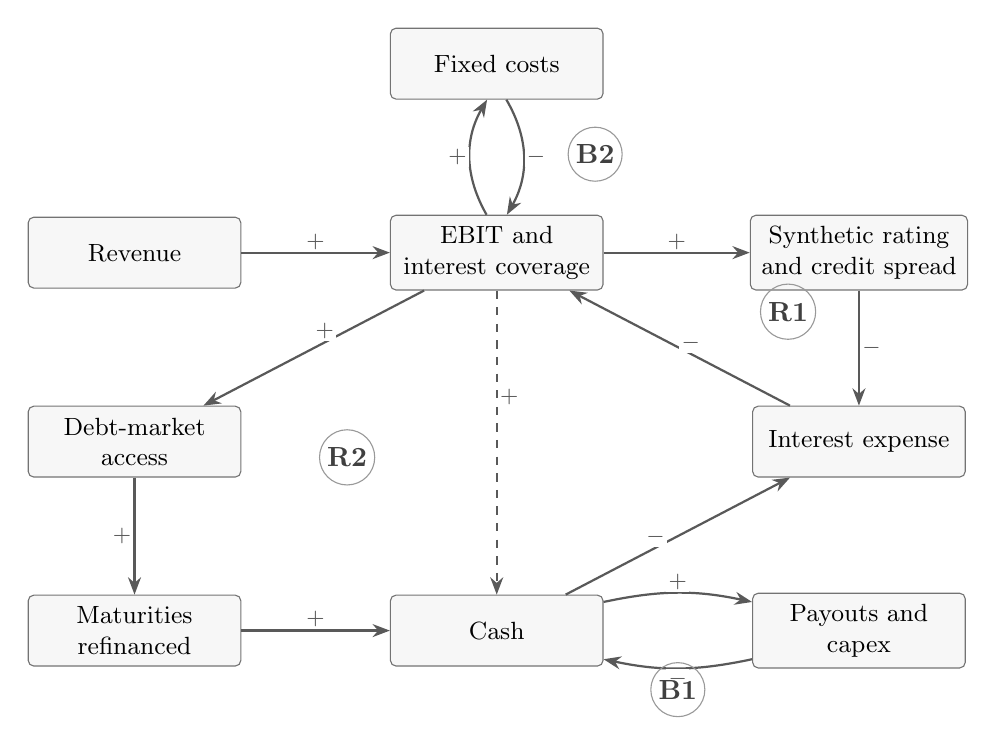
\begin{tikzpicture}[font=\small,
  var/.style={draw=black!55, rounded corners=2pt, fill=black!3, inner sep=4pt, align=center, minimum width=27mm, minimum height=9mm},
  arr/.style={-{Stealth[length=2.2mm]}, thick, black!65},
  lab/.style={font=\footnotesize, fill=white, inner sep=0.8pt},
  loop/.style={font=\bfseries, black!75, circle, draw=black!40, inner sep=1.5pt}]
% layout: a 3 x 4 grid; every loop is a closed cycle with the sign product shown in the caption
\node[var] (fixed) at (0, 2.4) {Fixed costs};
\node[var] (rev) at (-4.6, 0) {Revenue};
\node[var] (ebit) at (0, 0) {EBIT and\\interest coverage};
\node[var] (rating) at (4.6, 0) {Synthetic rating\\and credit spread};
\node[var] (access) at (-4.6, -2.4) {Debt-market\\access};
\node[var] (interest) at (4.6, -2.4) {Interest expense};
\node[var] (refi) at (-4.6, -4.8) {Maturities\\refinanced};
\node[var] (cash) at (0, -4.8) {Cash};
\node[var] (payouts) at (4.6, -4.8) {Payouts and\\capex};
\draw[arr] (rev) -- node[lab, above]{$+$} (ebit);
% R1: coverage -> rating -> interest -> coverage
\draw[arr] (ebit) -- node[lab, above]{$+$} (rating);
\draw[arr] (rating) -- node[lab, right]{$-$} (interest);
\draw[arr] (interest) -- node[lab, above, pos=0.45]{$-$} (ebit);
% R2: coverage -> access -> refinancing -> cash -> (revolver) interest -> coverage
\draw[arr] (ebit) -- node[lab, above, pos=0.45]{$+$} (access);
\draw[arr] (access) -- node[lab, left]{$+$} (refi);
\draw[arr] (refi) -- node[lab, above]{$+$} (cash);
\draw[arr] (cash) -- node[lab, above, pos=0.4]{$-$} (interest);
% B1: cash -> payouts and capex -> cash
\draw[arr] (cash.15) to[bend left=12] node[lab, above]{$+$} (payouts.165);
\draw[arr] (payouts.195) to[bend left=12] node[lab, below]{$-$} (cash.345);
% B2: margin -> fixed-cost cuts -> margin
\draw[arr] (ebit.105) to[bend left=30] node[lab, left]{$+$} (fixed.255);
\draw[arr] (fixed.285) to[bend left=30] node[lab, right]{$-$} (ebit.75);
\draw[arr, dashed] (ebit) -- node[lab, right, pos=0.35]{$+$} (cash);
\node[loop] at (3.7, -0.75) {R1};
\node[loop] at (-1.9, -2.6) {R2};
\node[loop] at (2.3, -5.55) {B1};
\node[loop] at (1.25, 1.25) {B2};
\end{tikzpicture}
\caption{The four feedback loops in causal-loop notation. A ``$+$'' (``$-$'') link means that the variables move in the same (opposite) direction; a loop is reinforcing (R) when the product of its signs is positive and balancing (B) when it is negative. R1, leverage--spread spiral: lower coverage worsens the rating, which raises interest and lowers coverage further. R2, market-access cliff: lower coverage reduces the share of maturities that can be refinanced, so cash falls, revolver drawings raise interest, and coverage falls further. B1, cash conservation: payouts and capex are cut as cash falls. B2, delayed restructuring: fixed costs are cut as margins fall. The dashed link (operating cash flow) is not part of a loop. The full model also contains working capital, customer deposits, the debt-maturity ladder, taxes and the recession regime.}
\label{fig:loops}
\end{figure}

\section{Evaluation design}\label{sec:design}

\subsection{Samples}
The universe is the current S\&P~500 outside Financials and Real Estate (394 companies), whose balance sheets fit a corporate cash-flow model, plus five former members or notable non-members that matter for 2020 (American Airlines, Macy's, Kohl's, Wynn Resorts, Intel); results without them are in Appendix Table~\ref{tab:robust}. A company enters a design when at least 16 quarters of filings are available at the cutoff, which rules out February 2013 because XBRL reporting began in 2009--2011. Because today's index members survived to today, we add a second sample of non-financial SEC registrants that filed for Chapter~11 between April and November 2020. It is a convenience sample of prominent filings, collected from public records and verified against the companies' XBRL filings, not an exhaustive census. Of 35 candidates, \BkN{} have the required history (Appendix Table~\ref{tab:bkfirms}); Valaris, Extraction Oil \& Gas, Garrett Motion, Ultra Petroleum and Pacific Drilling were listed or reorganized too recently. Energy companies, hit by the oil-price collapse, and retailers dominate the sample.

\subsection{Benchmarks}
Every benchmark is computed from the same point-in-time vintage as the twin. Eleven are classic: Altman's Z$''$-score for non-manufacturers \citep{altman2006}, Ohlson's O-score \citep{ohlson1980}, Zmijewski's score \citep{zmijewski1984}, interest coverage, net debt over EBITDA, cash over revenue, the current ratio, revenue volatility, the fixed-cost share estimated by the twin's calibration, size, and a \emph{static stress test}: the back-of-the-envelope calculation an analyst would do for the same scenario with the same inputs (liquidity divided by three quarters of fixed costs and interest, net of the contribution on the remaining revenue, plus debt maturing in those quarters). Two are cash-flow benchmarks that capture persistence: the trailing four-quarter free-cash-flow margin and capital expenditure over revenue. Finally, the \emph{health formula} applies the twin's scoring rule to the opening balance sheet, without any simulation. Because the health score combines runway, a coverage-based rating, leverage and Altman's Z$''$, comparing the twin with this formula isolates what the simulation adds to its own ingredients. We also fit a cross-validated composite of all thirteen benchmarks (ten folds, with sector effects). All predictors are oriented so that higher values mean higher risk.

\subsection{Outcomes}
\emph{Raw cash burn} is the worst cumulative free cash flow (operating cash flow less capital expenditure) over a window, as a percentage of revenue in the four quarters before the cutoff; worse than $-10\%$ is \emph{severe}. In the COVID design the window is 2020Q1--2021Q2. \emph{Abnormal cash burn} subtracts the company's trailing quarterly free-cash-flow run-rate from every quarter of the window before cumulating, so a utility that always invests more than it earns is not counted as stressed; it measures the deterioration the shock caused. In the panel, the twin is calibrated and simulated over twelve quarters, and outcomes cover the eight quarters after the last quarter known at the cutoff: severe raw and abnormal burn, \emph{coverage collapse} (trailing EBIT/interest falling below $1.5\times$, for companies above it at the cutoff), and a \emph{dividend cut} (dividends in the next four quarters below half of the previous four, for payers). Outcomes are measured on the latest data.

\subsection{The structural test}
To test transmission separately from the scenario, we replace the twin's simulated revenue with the revenue the company actually reported over the eight quarters after the cutoff, run 500 paths, take the median path of operating and free cash flow quarter by quarter, and record its worst cumulative value as a share of trailing revenue. Two rules see the same realized revenue: a \emph{margin rule} that applies the trailing operating- or free-cash-flow margin to it, and, for free cash flow, a \emph{run-rate} that ignores revenue. The margin rule is the natural null for a model whose purpose is to capture operating leverage, working capital and financing. Besides correlations with realized cash, we report the \emph{incremental correlation} between the twin's deviation from the margin rule and the realized deviation from it: whether the twin knows where pass-through fails.

\subsection{Inference}
Rank correlations and AUCs come with bootstrap confidence intervals (2{,}000 resamples; panel bootstraps resample firms). Comparisons between two predictors are paired, on the observations where both exist. Within-sector correlations correlate deviations of percentile ranks from GICS-sector means. Out-of-sample panel models are ridge-penalized logits with median imputation and missing-value indicators, winsorized at training-set percentiles; for test year $Y$ they are trained only on cutoffs up to $Y-3$, whose eight-quarter outcomes were reported by $Y$. Forecast comparisons use the CRPS scaled by mean quarterly revenue and Diebold--Mariano tests with standard errors clustered by firm and by forecast origin. We run many comparisons; individual $p$-values near 0.05 should be read with that in mind.

\section{Results}\label{sec:results}

\subsection{Ranking fragility before COVID-19}
Table~\ref{tab:covid} reports how well each predictor, frozen on 20 February 2020, ranks 2020--21 cash burn. The twin's stress score reaches $\rho$ = \CovRho{} (95\% CI \CovRhoLo--\CovRhoHi). It beats every classic benchmark: the best of them, \CovClassicName, reaches \CovClassicRho{} (paired difference \CovClassicDiff, $p\CovClassicP$), and the static stress test with the twin's own inputs reaches \CovStaticRho{} ($p\CovStaticP$). The advantage holds within sectors ($\rho$ = \CovWithin, 95\% CI \CovWithinLo--\CovWithinHi) and the twin's correlation is essentially unchanged without the five companies added for 2020 ($\rho$ = \CovNoAddedRho) and lower but positive without capital-intensive utilities ($\rho$ = \CovNoUtilRho; Appendix Table~\ref{tab:robust}). Simulating the demand-freeze scenario also improves on the health formula applied to the opening balance sheet ($\rho$ = \CovFormulaRho; difference \CovFormulaDiff, $p\CovFormulaP$) and on the twin's own baseline run ($\rho$ = \CovBaseRho; difference \CovStressBase, $p\CovStressBaseP$).

The cash-flow benchmarks change the picture. The trailing free-cash-flow margin alone ranks cash burn with $\rho$ = \CovFcfRho{} (95\% CI \CovFcfLo--\CovFcfHi, $n$ = \CovFcfN), well above the twin, also within sectors ($\rho$ = \CovFcfWithin), and the cross-validated composite of all benchmarks reaches \CovCompRho. In the rank regression of Table~\ref{tab:covidreg}, which includes every benchmark, the formula and sector effects, the twin's $t$-statistic is \CovRegT{} while the free-cash-flow margin's is \CovRegFcfT. Companies that burned cash in 2020--21 were, to a large extent, companies that burned cash before.

The abnormal-burn columns of Table~\ref{tab:covid} make the point directly. Measured against each company's own pre-2020 run-rate, the deterioration the shock caused is not ranked by the twin ($\rho$ = \AbnTwinRho, 95\% CI \AbnTwinLo--\AbnTwinHi), by Altman's Z$''$ ($\rho$ = \AbnAltmanRho), by the free-cash-flow margin ($\rho$ = \AbnFcfRho), or by the stress scenarios (Appendix Table~\ref{tab:scenarios}). Revenue volatility ($\rho$ = \AbnRevVolRho), capital intensity ($\rho$ = \AbnCapexRho) and the fixed-cost share ($\rho$ = \AbnFixedRho) carry modest signal, a composite fitted to all benchmarks reaches \AbnCompRho, and cash holdings are related with the opposite sign to the one a fragility measure would predict ($\rho$ = \AbnCashRho, 95\% CI \AbnCashLo--\AbnCashHi). The 2020 shock was concentrated in travel, leisure and energy for reasons --- a pandemic and an oil-price war --- that balance sheets do not reveal; a generic scenario applied to every company cannot recover them.

\begin{table}[t]
\centering\scriptsize
\setlength{\tabcolsep}{3.5pt}
\caption{Ranking 2020--21 cash burn with predictors frozen on 20 February 2020}
\label{tab:covid}
\begin{tabular}{lrrcrrrc}
\toprule
 & & \multicolumn{4}{c}{Raw cash burn} & \multicolumn{2}{c}{Abnormal cash burn} \\
\cmidrule(lr){3-6}\cmidrule(lr){7-8}
 & $n$ & $\rho$ & 95\% CI & Within sector & Twin $-$ predictor & $\rho$ & 95\% CI \\
\midrule
Twin: stress health score & 333 & 0.40 & [0.30, 0.49] & 0.29 &  & $-$0.02 & [$-$0.15, 0.11] \\
Twin: baseline health score & 333 & 0.35 & [0.24, 0.45] & 0.20 & +0.05$^{**}$ & 0.02 & [$-$0.10, 0.14] \\
Twin: breach probability & 333 & 0.31 & [0.22, 0.41] & 0.14 & +0.09$^{**}$ & $-$0.04 & [$-$0.16, 0.07] \\
Health formula, no simulation & 333 & 0.35 & [0.25, 0.45] & 0.23 & +0.05$^{**}$ & $-$0.02 & [$-$0.14, 0.10] \\
\addlinespace
Altman Z$''$ & 319 & 0.31 & [0.20, 0.41] & 0.21 & +0.11$^{***}$ & 0.04 & [$-$0.08, 0.17] \\
Ohlson O-score & 296 & 0.22 & [0.11, 0.33] & 0.13 & +0.21$^{***}$ & $-$0.01 & [$-$0.13, 0.11] \\
Zmijewski score & 317 & 0.17 & [0.05, 0.28] & 0.06 & +0.24$^{***}$ & 0.02 & [$-$0.11, 0.14] \\
Interest coverage & 333 & 0.27 & [0.17, 0.37] & 0.17 & +0.13$^{***}$ & 0.04 & [$-$0.08, 0.15] \\
Net debt / EBITDA & 333 & 0.23 & [0.12, 0.34] & 0.10 & +0.17$^{***}$ & $-$0.04 & [$-$0.16, 0.08] \\
Cash / revenue & 333 & 0.24 & [0.13, 0.35] & 0.11 & +0.16$^{***}$ & $-$0.18 & [$-$0.30, $-$0.06] \\
Current ratio & 325 & 0.23 & [0.12, 0.34] & 0.11 & +0.18$^{***}$ & $-$0.01 & [$-$0.13, 0.12] \\
Static stress test & 333 & 0.29 & [0.18, 0.40] & 0.17 & +0.11$^{***}$ & $-$0.09 & [$-$0.21, 0.03] \\
Revenue volatility & 333 & 0.19 & [0.08, 0.30] & 0.16 & +0.21$^{***}$ & 0.21 & [0.09, 0.32] \\
Fixed-cost share & 333 & 0.01 & [$-$0.10, 0.13] & $-$0.05 & +0.39$^{***}$ & 0.17 & [0.04, 0.29] \\
Size (log revenue) & 333 & $-$0.11 & [$-$0.22, 0.00] & $-$0.11 & +0.51$^{***}$ & 0.05 & [$-$0.06, 0.16] \\
\addlinespace
Trailing FCF margin & 292 & 0.68 & [0.59, 0.75] & 0.60 & $-$0.22$^{***}$ & $-$0.02 & [$-$0.15, 0.10] \\
Capex / revenue & 312 & 0.24 & [0.12, 0.35] & 0.10 & +0.20$^{***}$ & 0.21 & [0.09, 0.32] \\
\addlinespace
Cross-validated composite of all benchmarks & 333 & 0.64 & & & $-$0.24$^{***}$ & 0.36 & \\
\bottomrule
\end{tabular}

\par\smallskip
\begin{minipage}{\linewidth}\footnotesize
Spearman correlation between each risk-oriented predictor and realized burn severity across S\&P~500 non-financial companies. Raw burn: worst cumulative free cash flow in 2020Q1--2021Q2 as a share of trailing revenue (\CovSevere{} companies below $-10\%$). Abnormal burn: the same after subtracting each company's pre-2020 free-cash-flow run-rate (\AbnN{} companies with a run-rate). ``Within sector'' correlates deviations from GICS-sector means of percentile ranks. ``Twin $-$ predictor'': paired bootstrap difference in $\rho$ on the companies where both exist. $^{*}$, $^{**}$, $^{***}$: $p<0.10, 0.05, 0.01$.
\end{minipage}
\end{table}

\begin{figure}[t]
\centering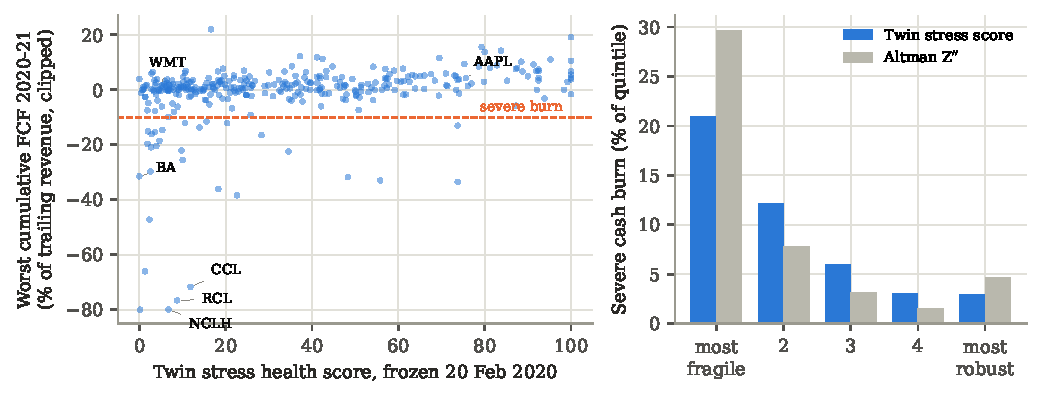
\includegraphics[width=\linewidth]{figures/covid.pdf}
\caption{Left: the twin's stress health score on 20 February 2020 against realized worst cumulative free cash flow in 2020--21. Right: share of companies with a severe cash burn by quintile of the twin's stress score and of Altman's Z$''$.}
\label{fig:covid}
\end{figure}

\begin{table}[t]
\centering\footnotesize
\begin{threeparttable}
\caption{Rank regression of 2020--21 raw cash-burn severity}
\label{tab:covidreg}
\begin{tabular}{lrr}
\toprule
Percentile rank of & Coefficient & ($t$, HC3) \\
\midrule
Twin: stress health score & 0.135 & (0.97) \\
Health formula, no simulation & $-$0.070 & ($-$0.49) \\
Altman Z$''$ & 0.022 & (0.22) \\
Ohlson O$-$score & 0.156 & (1.16) \\
Zmijewski score & $-$0.224 & ($-$1.69)$^{*}$ \\
Net debt / EBITDA & $-$0.042 & ($-$0.44) \\
Interest coverage & 0.007 & (0.07) \\
Cash / revenue & $-$0.162 & ($-$1.74)$^{*}$ \\
Current ratio & 0.161 & (2.10)$^{**}$ \\
Static stress test & $-$0.064 & ($-$0.56) \\
Revenue volatility & 0.084 & (1.53) \\
Fixed$-$cost share & 0.048 & (0.82) \\
Size (log revenue) & 0.039 & (0.59) \\
Trailing FCF margin & 0.634 & (8.89)$^{***}$ \\
Capex / revenue & 0.060 & (1.05) \\
\midrule
Sector fixed effects & \multicolumn{2}{r}{Yes} \\
$R^2$ (without the twin) & \multicolumn{2}{r}{0.50 (0.50)} \\
Observations & \multicolumn{2}{r}{333} \\
\bottomrule
\end{tabular}

\begin{tablenotes}\footnotesize
\item OLS of the percentile rank of realized burn severity on percentile ranks of the predictors (missing values at the median rank), with GICS sector fixed effects and HC3 standard errors. Benchmark coefficients are not interpretable individually because the benchmarks are strongly correlated.
\end{tablenotes}
\end{threeparttable}
\end{table}

\subsection{Companies that did not survive}
Table~\ref{tab:bankrupt} adds the \BkN{} companies that filed for Chapter~11 in 2020. Against all \BkSurv{} S\&P companies the twin's stress score separates them with an AUC of \BkAuc, but size alone reaches \BkSize, because index members are large. Restricting survivors to companies no larger than the 90th percentile of the bankrupt firms leaves \BkSmSurv{} survivors and \BkSmBk{} bankrupt firms. There the twin's AUC is \BkSmTwin{} (95\% CI \BkSmTwinLo--\BkSmTwinHi), against \BkSmAltman{} for Altman's Z$''$ (difference \BkSmTwinAltmanDiff, $p\BkSmTwinAltmanP$), \BkSmIcr{} for interest coverage ($p\BkSmTwinIcrP$), \BkSmFcf{} for the free-cash-flow margin ($p\BkSmTwinFcfP$; available for only \BkFcfBk{} bankrupt firms) and \BkSmSize{} for size. The health formula on the opening balance sheet, however, reaches \BkSmFormula{} (difference \BkSmTwinFormulaDiff, $p\BkSmTwinFormulaP$): what separates the bankruptcies is the combination of runway, coverage, leverage and solvency in the score, not the simulation. The stress scenario even hurts here: in the full sample the stress score is worse than the twin's baseline score (difference \BkStressBase, $p\BkStressBaseP$), possibly because a uniform demand freeze pushes many healthy companies toward the bottom of the scale and compresses the ranking. Two caveats apply: the bankrupt firms are a convenience sample, and the survivors survived until 2026, which makes them easier to separate than the 2020 population would have been.

\begin{table}[t]
\centering\footnotesize
\begin{threeparttable}
\caption{Chapter~11 filers of 2020 versus S\&P~500 survivors, predictors frozen on 20 February 2020}
\label{tab:bankrupt}
\resizebox{\linewidth}{!}{%
\begin{tabular}{lllll}
\toprule
 & \multicolumn{2}{c}{Panel 2014--2024, within 8 quarters} & \multicolumn{2}{c}{20 Feb 2020, to end-2021} \\
\cmidrule(lr){2-3}\cmidrule(lr){4-5}
 & All (377 events) & Already weak (311) & All (48) & Already weak (37) \\
\midrule
Twin: health score (panel: baseline; 2020: stress) & 0.86 [0.83, 0.88] & 0.77 [0.74, 0.80] & 0.86 [0.81, 0.91] & 0.76 [0.69, 0.82] \\
Twin: breach probability & 0.84 [0.82, 0.87] & 0.77 [0.74, 0.80] & 0.81 [0.76, 0.86] & 0.70 [0.64, 0.77] \\
Health formula, no simulation & 0.87 [0.85, 0.89] & 0.76 [0.73, 0.79] & 0.85 [0.80, 0.90] & 0.72 [0.65, 0.79] \\
\addlinespace
Altman Z$''$ & 0.81 [0.79, 0.83] & 0.66 [0.63, 0.69] & 0.80 [0.74, 0.84] & 0.59 [0.52, 0.66] \\
Ohlson O-score & 0.86 [0.83, 0.87] & 0.76 [0.73, 0.79] & 0.79 [0.71, 0.87] & 0.70 [0.61, 0.79] \\
Zmijewski score & 0.82 [0.80, 0.85] & 0.75 [0.72, 0.78] & 0.78 [0.71, 0.85] & 0.73 [0.65, 0.80] \\
Interest coverage & 0.79 [0.77, 0.82] & 0.64 [0.61, 0.67] & 0.76 [0.70, 0.82] & 0.60 [0.53, 0.68] \\
Net debt / EBITDA & 0.78 [0.76, 0.81] & 0.66 [0.63, 0.69] & 0.75 [0.68, 0.81] & 0.61 [0.52, 0.69] \\
Cash / revenue & 0.61 [0.57, 0.64] & 0.59 [0.55, 0.63] & 0.64 [0.57, 0.72] & 0.65 [0.56, 0.73] \\
Current ratio & 0.68 [0.65, 0.72] & 0.62 [0.59, 0.65] & 0.71 [0.65, 0.78] & 0.64 [0.57, 0.72] \\
Static stress test & 0.78 [0.75, 0.81] & 0.71 [0.68, 0.75] & 0.78 [0.72, 0.84] & 0.67 [0.60, 0.74] \\
Revenue volatility & 0.65 [0.61, 0.70] & 0.58 [0.54, 0.62] & 0.61 [0.52, 0.70] & 0.53 [0.43, 0.64] \\
Fixed-cost share & 0.66 [0.62, 0.70] & 0.61 [0.58, 0.65] & 0.70 [0.61, 0.77] & 0.62 [0.53, 0.71] \\
Size (log revenue) & 0.62 [0.58, 0.65] & 0.50 [0.46, 0.54] & 0.57 [0.50, 0.64] & 0.39 [0.32, 0.48] \\
\addlinespace
Trailing FCF margin & 0.80 [0.78, 0.83] & 0.60 [0.56, 0.64] & 0.78 [0.71, 0.84] & 0.54 [0.43, 0.64] \\
Capex / revenue & 0.51 [0.46, 0.55] & 0.50 [0.45, 0.54] & 0.49 [0.38, 0.59] & 0.50 [0.40, 0.61] \\
\bottomrule
\end{tabular}}

\begin{tablenotes}\footnotesize
\item AUC for separating 2020 Chapter~11 filers from S\&P~500 non-financial companies. Paired differences use the companies where both predictors exist. Size-matched: survivors no larger than the 90th percentile of bankrupt firms' revenue. $^{*}$, $^{**}$, $^{***}$: $p<0.10, 0.05, 0.01$.
\end{tablenotes}
\end{threeparttable}
\end{table}

\begin{figure}[t]
\centering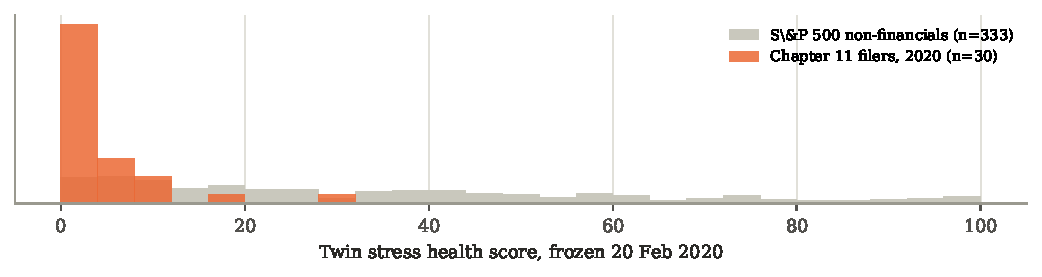
\includegraphics[width=\linewidth]{figures/bankrupt.pdf}
\caption{Distribution of the twin's stress health score on 20 February 2020 for S\&P~500 non-financial companies and for companies that filed for Chapter~11 in 2020.}
\label{fig:bankrupt}
\end{figure}

\subsection{Translating a shock into cash}
Table~\ref{tab:structural} reports the structural test. In 2020, among the \StrCovDownN{} companies whose revenue over the eight quarters after the cutoff fell by more than 10\%, the twin's simulated operating cash flow correlates with the realized one at $\rho$ = \StrCovDownCfoTwin, against \StrCovDownCfoMargin{} for the margin rule ($p\StrCovDownCfoP$); for free cash flow the figures are \StrCovDownFcfTwin{} and \StrCovDownFcfMargin{} ($p\StrCovDownFcfP$). When revenue collapses, the cash response is shaped by fixed costs, working-capital releases, customer-deposit refunds and maturing debt, which a proportional rule ignores and the twin models. Carnival is the extreme case: with its realized revenue, the twin reproduces the timing and shape of the collapse in free cash flow but understates its depth (Figure~\ref{fig:ccl}).

This advantage does not generalize to all revenue declines: across the \StrPanDownN{} firm-years of the 2014--2023 panel with such declines, twin and rule are level ($\rho$ = \StrPanDownCfoTwin{} against \StrPanDownCfoMargin). Over the whole panel (\StrPanN{} firm-years of \StrPanFirms{} companies), the margin rule is better in levels: its median absolute error is \StrPanMaeMargin{} percentage points of revenue against \StrPanMaeTwin{} for the twin, and the twin is closer in \StrPanCloser{} of cases. But the twin knows where the rule goes wrong. The correlation between the twin's deviation from the rule and the realized deviation is \StrPanIncr{} (95\% CI \StrPanIncrLo--\StrPanIncrHi), and it is positive in every year, from \StrPanYearMin{} in \StrPanYearMinYear{} to \StrPanYearMax{} (Figure~\ref{fig:structural}). The practical implication is a combination: the margin rule for the level, and the twin for the direction and size of departures from it.

\begin{table}[t]
\centering\scriptsize
\setlength{\tabcolsep}{3.5pt}
\caption{The structural test: realized revenue fed into the twin}
\label{tab:structural}
\begin{tabular}{llrrrrlr}
\toprule
 & & & \multicolumn{3}{c}{$\rho$ with realized cash} & Incremental $\rho$ & Median abs.\ error \\
\cmidrule(lr){4-6}
Sample & Cash measure & $n$ & Twin & Margin rule & Difference & [95\% CI] & twin / rule (pp) \\
\midrule
2020, all companies & Operating cash flow & 281 & 0.66 & 0.63 & +0.03 & 0.35 [0.22, 0.46] & 2.0 / 1.5 \\
2020, all companies & Free cash flow & 281 & 0.66 & 0.73 & $-$0.07 & 0.36 [0.23, 0.48] & 2.3 / 1.7 \\
\addlinespace
2020, revenue down $>$10\% & Operating cash flow & 48 & 0.72 & 0.27 & +0.45$^{***}$ & 0.41 [0.09, 0.66] & 2.9 / 2.3 \\
2020, revenue down $>$10\% & Free cash flow & 48 & 0.76 & 0.51 & +0.25$^{***}$ & 0.55 [0.27, 0.76] & 3.9 / 3.0 \\
\addlinespace
2014--2023, all firm-years & Operating cash flow & 2{,}661 & 0.60 & 0.66 & $-$0.06$^{***}$ & 0.30 [0.25, 0.36] & 1.9 / 1.5 \\
2014--2023, all firm-years & Free cash flow & 2{,}661 & 0.57 & 0.67 & $-$0.10$^{***}$ & 0.30 [0.25, 0.35] & 2.2 / 1.8 \\
\addlinespace
2014--2023, revenue down $>$10\% & Operating cash flow & 331 & 0.54 & 0.53 & +0.01 & 0.22 [0.09, 0.33] & 2.6 / 1.6 \\
2014--2023, revenue down $>$10\% & Free cash flow & 331 & 0.50 & 0.51 & $-$0.02 & 0.19 [0.06, 0.32] & 3.5 / 2.1 \\
\bottomrule
\end{tabular}

\par\smallskip
\begin{minipage}{\linewidth}\footnotesize
Worst cumulative operating or free cash flow over the eight quarters after the cutoff, as a share of trailing revenue, with the realized revenue of those quarters given to the twin and to the margin rule (trailing cash-flow margin times realized revenue). ``Difference'': paired bootstrap difference in $\rho$ (panel: clustered by firm). Incremental $\rho$: correlation of (twin $-$ rule) with (realized $-$ rule). 2020 cutoff: 20 February 2020; panel cutoffs: 15 February 2014--2023. $^{*}$, $^{**}$, $^{***}$: $p<0.10, 0.05, 0.01$.
\end{minipage}
\end{table}

\begin{figure}[t]
\centering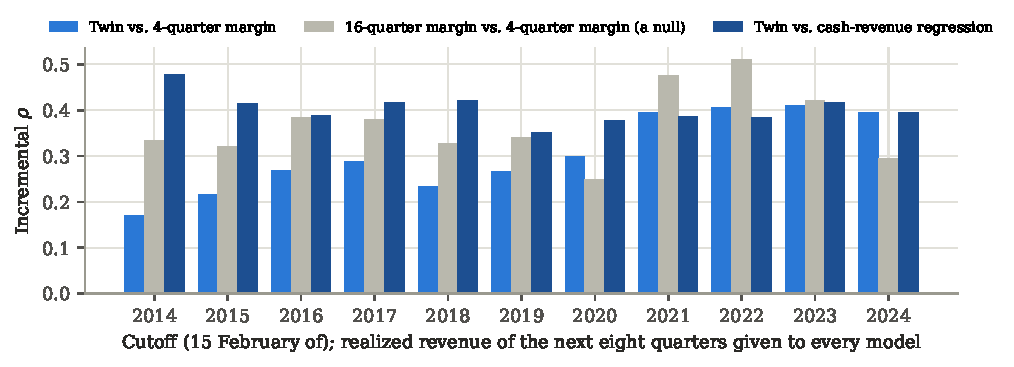
\includegraphics[width=\linewidth]{figures/structural.pdf}
\caption{Incremental correlation between the twin's and the realized departure of operating cash flow from the margin rule, by cutoff year (bars), and its pooled 95\% confidence interval (band).}
\label{fig:structural}
\end{figure}

\subsection{A decade of distress}
Table~\ref{tab:panel} summarizes \PanFirmYears{} firm-years of \PanFirms{} companies with cutoffs from \PanYears. The twin's baseline health score predicts severe raw cash burn over the next eight quarters with an AUC of \PanTwinAuc, above the health formula (\PanFormulaAuc, $p\PanFormulaP$), Altman's Z$''$ (\PanAltmanAuc) and interest coverage (\PanIcrAuc), but below the trailing free-cash-flow margin (\PanFcfAuc). Out of sample (test years \PanOosYears), a logit with all benchmarks and the formula reaches \PanOosBench{}, and adding the twin changes it by \PanOosDelta. For abnormal burn the twin has no skill (AUC \PanAbnTwinAuc); for coverage collapse, the current coverage ratio is the best predictor; and for dividend cuts the twin is comparable with the benchmarks without adding to them. Year by year (Figure~\ref{fig:panel}), the free-cash-flow margin is the best predictor in \PanFcfBestYears{} of \PanYearCount{} years, and Altman's Z$''$ beats the twin in 2014, 2015 and 2017.

\begin{table}[t]
\centering\scriptsize
\setlength{\tabcolsep}{4pt}
\caption{Distress over the next eight quarters, \PanYears{} panel}
\label{tab:panel}
\resizebox{\linewidth}{!}{%
\begin{tabular}{lrrrrlrrl}
\toprule
 & & & \multicolumn{3}{c}{Univariate AUC} & \multicolumn{3}{c}{Out-of-sample logit AUC} \\
\cmidrule(lr){4-6}\cmidrule(lr){7-9}
Event (next 8 quarters) & Firm-years & Events & Twin & Formula & Best benchmark & Benchmarks & + Twin & $\Delta$ [95\% CI] \\
\midrule
Severe cash burn & 19{,}019 & 2{,}856 & 0.72 & 0.71 & 0.82 (trailing FCF margin) & 0.87 & 0.87 & +0.002 [0.001, 0.004]$^{***}$ \\
Severe abnormal burn & 16{,}033 & 3{,}730 & 0.52 & 0.51 & 0.62 (revenue volatility) & 0.68 & 0.68 & $-$0.004 [$-$0.007, $-$0.001]$^{**}$ \\
Coverage collapse & 9{,}120 & 1{,}953 & 0.58 & 0.59 & 0.66 (interest coverage) & 0.69 & 0.70 & +0.005 [0.002, 0.008]$^{***}$ \\
Dividend cut & 8{,}794 & 766 & 0.69 & 0.69 & 0.69 (Ohlson O-score) & 0.74 & 0.75 & +0.002 [$-$0.004, 0.008] \\
Bankruptcy petition & 21{,}368 & 420 & 0.86 & 0.87 & 0.86 (Ohlson O-score) & 0.87 & 0.87 & +0.000 [$-$0.009, 0.008] \\
\bottomrule
\end{tabular}}

\par\smallskip
\begin{minipage}{\linewidth}\footnotesize
Twin: baseline health score (no stress scenario). Formula: the health formula on the opening balance sheet. Out-of-sample logits are ridge-penalized and trained for each test year on cutoffs at least three years earlier; ``Benchmarks'' contains all thirteen benchmarks and the formula, and ``+ Twin'' adds the twin's baseline health, baseline breach probability and recession-scenario health. $\Delta$: difference in AUC with a firm-clustered paired bootstrap CI. $^{*}$, $^{**}$, $^{***}$: $p<0.10, 0.05, 0.01$.
\end{minipage}
\end{table}

\begin{figure}[t]
\centering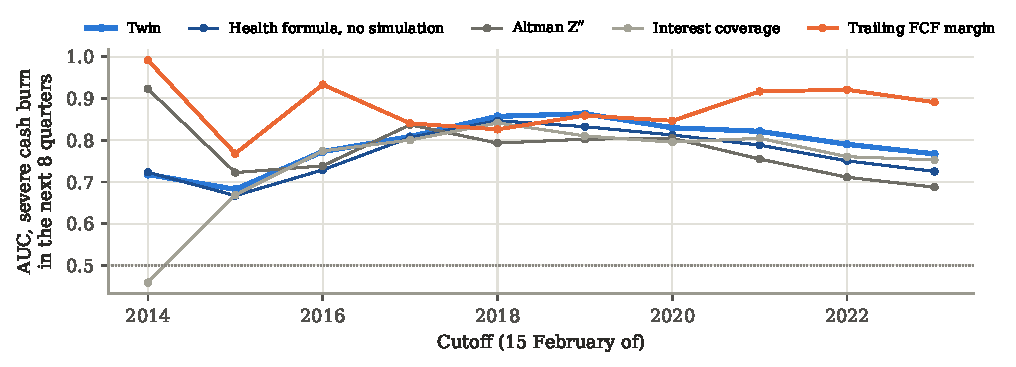
\includegraphics[width=\linewidth]{figures/panel_auc.pdf}
\caption{AUC for severe raw cash burn in the next eight quarters, by cutoff year.}
\label{fig:panel}
\end{figure}

\subsection{Feedback loops}
Table~\ref{tab:ablations} switches off each loop. The ranking by stress health barely changes, even without any loop (change \AblHealthLoss, $p\AblHealthP$), and in the panel a twin without loops predicts cash burn just as well (AUC \PanNoLoopsAuc{} against \PanTwinAuc). The loops matter more for the breach probability: for raw burn, removing the market-access cliff (R2) lowers its correlation by \AblRtwoLoss{} ($p\AblRtwoP$). For abnormal burn the same ablation goes the other way (\AblAbnRtwoLoss, $p\AblAbnRtwoP$). Given the number of comparisons, we read this as no reliable evidence that the loops improve rankings. Their role is in scenario analysis --- they determine whether and when a stressed company runs out of cash --- which a cross-sectional ranking test does not measure.

\begin{table}[t]
\centering\scriptsize
\setlength{\tabcolsep}{3.5pt}
\begin{threeparttable}
\caption{Loop ablations, COVID cross-section}
\label{tab:ablations}
\begin{tabular}{lrrrrrrrr}
\toprule
 & \multicolumn{6}{c}{Raw cash burn} & \multicolumn{2}{c}{Abnormal burn} \\
\cmidrule(lr){2-7}\cmidrule(lr){8-9}
 & \multicolumn{4}{c}{8 quarters} & \multicolumn{2}{c}{12 quarters} & \multicolumn{2}{c}{8 quarters} \\
\cmidrule(lr){2-5}\cmidrule(lr){6-7}\cmidrule(lr){8-9}
 & $\rho$(health) & loss & $\rho$(breach) & loss & $\rho$(breach) & loss & $\rho$(breach) & loss \\
\midrule
All loops (full twin) & 0.403 &  & 0.310 &  & 0.329 &  & $-$0.042 &  \\
without R1 (spread spiral) & 0.402 & +0.000 & 0.319 & $-$0.009 & 0.326 & +0.003 & $-$0.011 & $-$0.031$^{*}$ \\
without R2 (market-access cliff) & 0.394 & +0.009$^{*}$ & 0.230 & +0.079$^{**}$ & 0.253 & +0.078$^{**}$ & 0.072 & $-$0.116$^{**}$ \\
without B1 (cash conservation) & 0.404 & $-$0.001 & 0.299 & +0.011 & 0.300 & +0.029 & $-$0.069 & +0.027 \\
without B2 (restructuring) & 0.404 & $-$0.002 & 0.304 & +0.007 & 0.339 & $-$0.009 & $-$0.062 & +0.019 \\
without any loop & 0.395 & +0.007 & 0.236 & +0.074$^{**}$ & 0.255 & +0.074$^{*}$ & 0.095 & $-$0.138$^{***}$ \\
\bottomrule
\end{tabular}

\begin{tablenotes}\footnotesize
\item Spearman correlation between versions of the twin under the demand-freeze scenario and realized 2020--21 burn severity. ``Loss'': paired bootstrap difference between the full and the ablated twin (positive: the loop helps). $^{*}$, $^{**}$, $^{***}$: $p<0.10, 0.05, 0.01$.
\end{tablenotes}
\end{threeparttable}
\end{table}

\subsection{Forecast accuracy and calibration}
Table~\ref{tab:fc} compares the twin's four-quarter predictive distributions with a seasonal random walk with historical spread and with an ETS model \citep{hyndman2008} (additive errors, damped trend and seasonality on log revenue; simple exponential smoothing for cash), on \FcRevN{} revenue forecast--horizon pairs (about \FcRevFc{} four-quarter forecasts). The twin's scaled CRPS for revenue is \FcRevRw{} lower than the random walk's and \FcRevEts{} lower than ETS's (two-way clustered $t$ = \FcRevRwT{} and \FcRevEtsT). For cash, both benchmarks are better (skill \FcCashRw{} and \FcCashEts): treasury decisions are discretionary, and the twin models them as noise around policies inferred from history.

Raw predictive intervals are too narrow (Figure~\ref{fig:cal}). In the weekly validation run of the software, which pools \NForecasts{} revenue and cash forecast--horizon pairs, the nominal 90\% revenue interval covers \RevRawNinety{} of outcomes; online split-conformal rescaling \citep{vovk2005,gibbs2021}, using only errors from earlier cutoffs, restores coverage to \RevConfNinety{} for revenue and \CashConfNinety{} for cash.

\begin{table}[t]
\centering\scriptsize
\setlength{\tabcolsep}{3.5pt}
\begin{threeparttable}
\caption{Four-quarter probabilistic forecasts}
\label{tab:fc}
\begin{tabular}{lrrrrrrrrrr}
\toprule
 & & & \multicolumn{4}{c}{vs.\ seasonal random walk} & \multicolumn{4}{c}{vs.\ ETS} \\
\cmidrule(lr){4-7}\cmidrule(lr){8-11}
 & Pairs & Firms & Skill & Pooled & Better & DM $t$ & Skill & Pooled & Better & DM $t$ \\
\midrule
Revenue & 15{,}112 & 374 & 27\% & 28\% & 69\% & $-$5.84 & 18\% & 15\% & 58\% & $-$3.38 \\
Cash and short-term investments & 15{,}267 & 377 & $-$29\% & $-$25\% & 44\% & 5.06 & $-$36\% & $-$31\% & 40\% & 5.90 \\
\bottomrule
\end{tabular}

\begin{tablenotes}\footnotesize
\item Pairs: forecast--horizon pairs for which all three models produced a distribution. Skill: $1-\overline{\mathrm{CRPS}}_{\text{twin}}/\overline{\mathrm{CRPS}}_{\text{benchmark}}$ with each CRPS scaled by mean quarterly revenue; pooled: in unscaled dollars. Better: share of pairs where the twin's CRPS is lower. DM $t$: Diebold--Mariano statistic on scaled CRPS differences, clustered by firm and origin (negative: the twin is better).
\end{tablenotes}
\end{threeparttable}
\end{table}

\begin{figure}[t]
\centering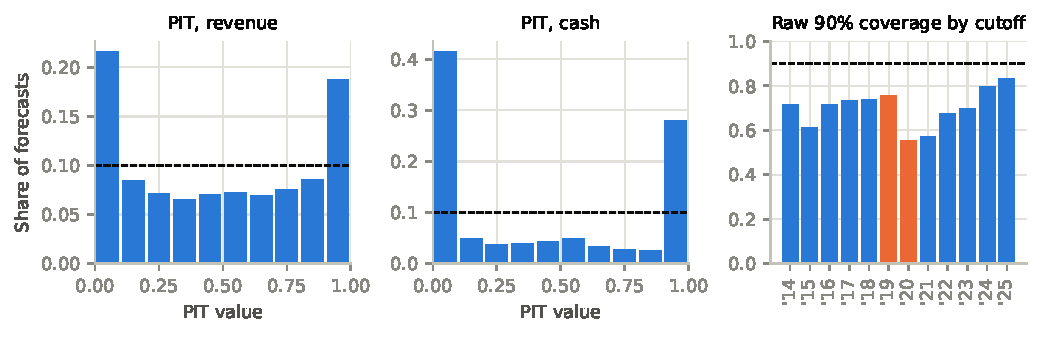
\includegraphics[width=\linewidth]{figures/calibration.pdf}
\caption{Probability integral transform histograms of the twin's raw forecasts (dashed: uniform) and raw 90\% interval coverage by cutoff year, from the weekly validation run. The U-shape shows that raw intervals are too narrow; cutoffs whose window contains the 2020 shock are the worst.}
\label{fig:cal}
\end{figure}

\begin{figure}[t]
\centering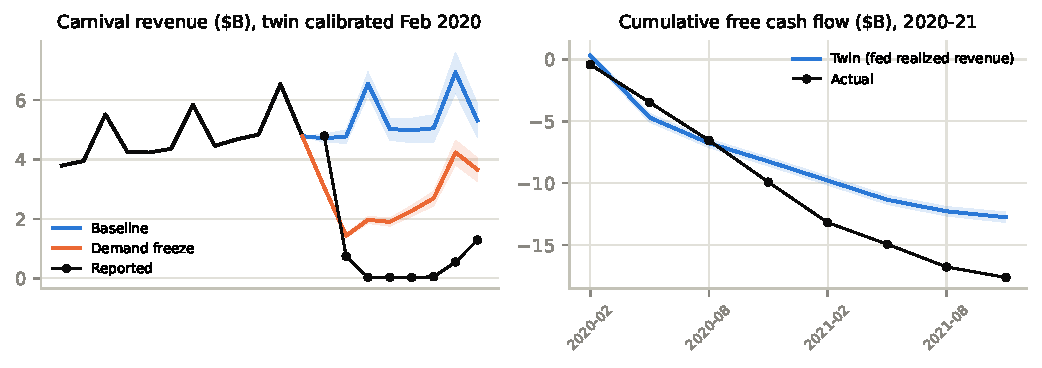
\includegraphics[width=\linewidth]{figures/carnival.pdf}
\caption{Carnival. Left: revenue forecasts of the twin frozen in February 2020 under the baseline and the demand-freeze scenario, against reported revenue. Right: the structural test for Carnival, with realized revenue fed into the twin (cumulative free cash flow \StructCCLCovidModel{} simulated against \StructCCLCovidActual{} realized, quarterly correlation \StructCCLCovidCorr).}
\label{fig:ccl}
\end{figure}

\section{Discussion and limitations}\label{sec:discussion}

\paragraph{What a twin is for.} The evidence separates the two halves of a stress test. Ranking companies by fragility under a generic scenario mostly reproduces what persistent cash-flow characteristics already reveal, and neither the twin nor the classic distress scores anticipated who the 2020 shock would hit. Translating a given shock into cash is different: there the simulated mechanics add information about departures from a proportional rule, consistently over ten years, although the rule remains the better point estimate. A filing-based twin is therefore most useful where the shock is specified --- scenario analysis, planning, covenant and liquidity headroom under a stated path for revenue --- and least useful as an unconditional early-warning score. Figure~\ref{fig:ccl} illustrates both halves for Carnival.

\paragraph{Evaluating stress and distress models.} Two controls changed our conclusions and should be routine: a persistence benchmark such as the trailing free-cash-flow margin, and an outcome measured against each company's own run-rate. Without them, our initial results suggested that the twin anticipated who would bleed in 2020; with them, the ranking evidence largely disappears.

\paragraph{Hindsight and data.} Several design choices were made after 2020: the demand-freeze scenario resembles the 2020 shock, the health-score weights and shrinkage priors were set during development, and the rating table is the January 2026 version of \citet{damodaran2026}, applied to earlier cutoffs. Macroeconomic inputs use final rather than real-time vintages. These choices favour the twin, which strengthens the negative findings and qualifies the positive ones. The main universe consists of today's index members, which creates survivorship bias; the bankruptcy sample addresses it only for 2020 and is not exhaustive. Some XBRL items are tagged idiosyncratically, missing quarters in outcome windows are treated as zero cash flow or no dividend (in the abnormal-burn measure, as the run-rate), and some parameters (for example undrawn credit lines when untagged) are assumptions.

\paragraph{Outcomes and scope.} Cash burn is not distress, and defaults, downgrades or covenant breaches would be better outcomes but are not available from filings. The structural test uses realized revenue, so it cannot separate the model's mechanics from errors in the reported revenue path itself. The product version of the health score also scores coverage and leverage against sector norms estimated from current data; it is excluded from the evaluation, and with it the 2020 raw-burn correlation is \CovSectorAdj.

\section{Conclusion}\label{sec:conclusion}

A transparent stock-and-flow model of the firm, calibrated automatically from public filings and evaluated without look-ahead, does not tell us in advance who a crisis will hit: once persistence is controlled for, neither it nor the classic distress scores ranked the 2020 shock. What it does is identify where a proportional rule misjudges the cash response to a given shock, consistently across a decade of out-of-sample tests, and forecast revenue better than standard time-series benchmarks. That is the job a stress test is for. Because the twin runs in a web browser and every number in this paper is generated from open code, the tests can be repeated and extended --- with market-based inputs, industry-specific scenarios and outcomes such as defaults --- by anyone.

\section*{Data and code availability}
All code, the point-in-time data pipeline, the research experiments and the scripts that generate every table, figure and number in this paper are available at \url{https://github.com/SpiliosDimakopoulos/fintwin} under the MIT licence, with an archived version on Zenodo. The experiments run on free GitHub-hosted runners (\texttt{.github/workflows/research.yml}). An interactive version of the twin, which recomputes 5{,}000 Monte Carlo paths in the browser, is at \url{https://spiliosdimakopoulos.github.io/fintwin/}. All inputs are public: SEC EDGAR XBRL filings and FRED.

\section*{Use of AI tools}
Software development, data analysis and drafting were assisted by an AI coding assistant (Claude, Anthropic), and an AI-generated referee report was used to identify weaknesses in an earlier version. The author designed the study, reviewed all code, results and text, and takes full responsibility for the content.

\bibliographystyle{plainnat}
\bibliography{references}

\appendix
\section{Additional tables and figures}

\begin{table}[h]
\centering\small
\caption{COVID cross-section: Spearman correlation of the twin's health score under each scenario with realized 2020--21 burn severity}
\label{tab:scenarios}
\begin{tabular}{lrrrrrr}
\toprule
 & Baseline & Rates +200bp & Sales $-$20\% & Recession & Credit crunch & Demand freeze \\
\midrule
Raw burn & 0.35 & 0.35 & 0.36 & 0.37 & 0.35 & 0.40 \\
Abnormal burn & 0.02 & 0.02 & 0.01 & 0.01 & 0.03 & $-$0.02 \\
\bottomrule
\end{tabular}

\end{table}

\begin{table}[h]
\centering\small
\caption{Robustness of the 2020 raw-burn ranking}
\label{tab:robust}
\begin{tabular}{lrrrlr}
\toprule
Sample & $n$ & Twin (stress) & Twin (baseline) & Best benchmark & $\rho$ \\
\midrule
Without the five added companies & 328 & 0.40 & 0.35 & trailing FCF margin & 0.68 \\
Without utilities & 308 & 0.35 & 0.27 & trailing FCF margin & 0.64 \\
\bottomrule
\end{tabular}

\end{table}

\begin{table}[h]
\centering\scriptsize
\caption{Calibrated parameters}
\label{tab:params}
\begin{tabular}{lp{0.5\linewidth}l}
\toprule
Parameter & Estimate & Window \\
\midrule
Seasonal factors $S_q$ & median ratio to centred 4-quarter moving average & last 32 quarters \\
Trend growth $\mu$ & median log growth, shrunk 50\% toward 1.2\%/quarter & last 12 quarters \\
AR coefficient $\phi$, volatility $\sigma_g$ & OLS; median absolute deviation of residuals & last 32 quarters \\
Tail index & Student-$t$ maximum likelihood on standardized residuals & growth residuals \\
Cyclicality $\beta$ & regression of revenue on nominal GDP growth, shrunk 50\% toward 1.5 & last 40 quarters \\
Recession entry and exit & NBER recessions since 1947 & FRED \\
Fixed costs $F$, variable ratio $v$ & penalized regression of cash costs on revenue & last 16 quarters \\
Margin shock $m_t$ & AR(1) of cost-regression residuals; correlation with demand & last 16 quarters \\
DSO, DIO, DPO, deposit days & averages of balance to revenue or costs & last 4 quarters \\
Depreciation, capex, SBC ratios & medians & last 8 quarters \\
Coupon & interest expense over debt & last 4 quarters \\
Rollover share & two-year debt trend relative to maturities & last 8 quarters \\
Discretionary financing volatility & robust s.d.\ of quarterly debt changes & last 20 quarters \\
Maturity ladder & XBRL maturity schedule, else six-year average life & latest 10-K \\
Credit facility & XBRL facility size, else 8\% of revenue (assumption) & latest filing \\
Minimum cash & half the 10th-percentile cash balance & last 12 quarters \\
Short-rate dynamics & Vasicek fit to the 3-month Treasury bill & since 2000 \\
\bottomrule
\end{tabular}
\end{table}

\begin{table}[h]
\centering\scriptsize
\caption{Companies that filed for Chapter~11 in 2020, ordered by the twin's stress health score on 20 February 2020}
\label{tab:bkfirms}
\begin{tabular}{llcrr}
\toprule
Company & Sector & Chapter 11 & Stress health & Baseline health \\
\midrule
Global Eagle Entertainment & Communication Services & 2020-07 & 0.0 & 0.5 \\
Pyxus International & Consumer Staples & 2020-06 & 0.0 & 1.1 \\
J.Crew Group & Consumer Discretionary & 2020-05 & 0.1 & 3.9 \\
Diamond Offshore Drilling & Energy & 2020-04 & 0.4 & 0.9 \\
Chesapeake Energy & Energy & 2020-06 & 0.4 & 2.1 \\
Hertz Global Holdings & Industrials & 2020-05 & 0.5 & 41.0 \\
Ascena Retail Group & Consumer Discretionary & 2020-07 & 0.5 & 4.6 \\
Tuesday Morning & Consumer Discretionary & 2020-05 & 0.6 & 4.4 \\
CEC Entertainment & Consumer Discretionary & 2020-06 & 0.8 & 8.2 \\
California Resources & Energy & 2020-07 & 0.8 & 2.4 \\
Tailored Brands & Consumer Discretionary & 2020-08 & 1.1 & 10.3 \\
Mallinckrodt & Health Care & 2020-10 & 1.1 & 11.4 \\
Stage Stores & Consumer Discretionary & 2020-05 & 1.7 & 44.5 \\
Akorn & Health Care & 2020-05 & 1.7 & 7.4 \\
Whiting Petroleum & Energy & 2020-04 & 1.9 & 13.0 \\
Frontier Communications & Communication Services & 2020-04 & 2.1 & 10.9 \\
Superior Energy Services & Energy & 2020-09 & 2.3 & 2.8 \\
Gulfport Energy & Energy & 2020-11 & 2.6 & 8.4 \\
Libbey & Consumer Discretionary & 2020-06 & 3.3 & 12.2 \\
Denbury Resources & Energy & 2020-07 & 3.7 & 14.1 \\
Intelsat & Communication Services & 2020-05 & 4.1 & 12.0 \\
Hi-Crush & Energy & 2020-07 & 4.2 & 15.4 \\
J. C. Penney Company & Consumer Discretionary & 2020-05 & 4.7 & 8.9 \\
GNC Holdings & Consumer Discretionary & 2020-06 & 5.2 & 46.1 \\
Briggs \& Stratton & Industrials & 2020-07 & 5.7 & 5.1 \\
Oasis Petroleum & Energy & 2020-09 & 8.7 & 56.3 \\
Unit Corporation & Energy & 2020-05 & 10.0 & 15.4 \\
Noble Corporation & Energy & 2020-07 & 11.0 & 42.9 \\
Hornbeck Offshore Services & Energy & 2020-05 & 19.0 & 56.7 \\
Chaparral Energy & Energy & 2020-08 & 30.0 & 30.0 \\
\bottomrule
\end{tabular}

\end{table}

\begin{figure}[h]
\centering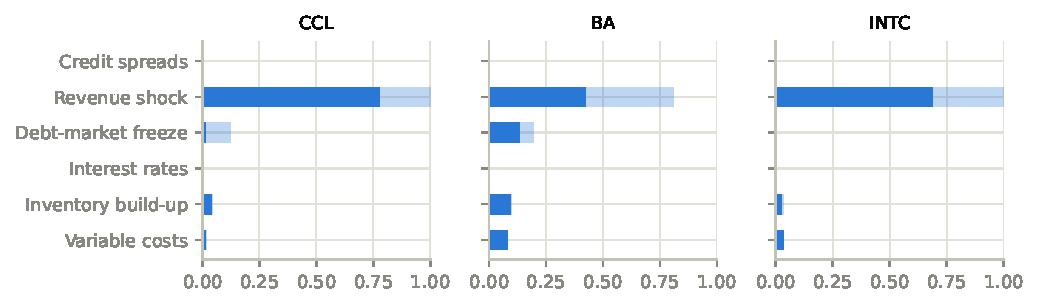
\includegraphics[width=0.9\linewidth]{figures/sobol.pdf}
\caption{Sobol indices of the health score for a representative company over the joint scenario space (solid: first-order; light: total). Large gaps indicate interactions: a debt-market freeze matters mainly together with a revenue shock.}
\label{fig:sobol}
\end{figure}

\section{Implementation}
The Python reference engine (NumPy) performs calibration, experiments and exports. A line-for-line TypeScript port runs in a Web Worker, so the public dashboard needs no server. Golden runs exported from Python with identical pre-drawn shocks must agree to $10^{-6}$ on eleven output series, the balance-sheet identity is checked by property-based tests, and the data pipeline is tested end to end on synthetic XBRL. The data are rebuilt weekly on free GitHub-hosted runners.

\end{document}
